\documentclass[12pt,a4paper]{report}

% ============== PACKAGES ==============
\usepackage[utf8]{inputenc}
\usepackage[T1]{fontenc}
\usepackage{geometry}
\usepackage{graphicx}
\usepackage{xcolor}
\usepackage{titlesec}
\usepackage{fancyhdr}
\usepackage{hyperref}
\usepackage{listings}
\usepackage{tcolorbox}
\usepackage{booktabs}
\usepackage{array}
\usepackage{multirow}
\usepackage{tikz}
\usepackage{forest}
\usepackage{algorithm}
\usepackage{algpseudocode}
\usepackage{amsmath}
\usepackage{enumitem}
\usepackage{tocloft}

\usetikzlibrary{shapes.geometric, arrows, positioning, calc}

% ============== PAGE SETUP ==============
\geometry{margin=1in}
\setlength{\parindent}{0pt}
\setlength{\parskip}{6pt}

% ============== COLORS ==============
\definecolor{primaryblue}{RGB}{0, 102, 153}
\definecolor{secondaryblue}{RGB}{51, 153, 204}
\definecolor{codebg}{RGB}{245, 245, 245}
\definecolor{codegreen}{RGB}{0, 128, 0}
\definecolor{codepurple}{RGB}{128, 0, 128}

% ============== HYPERREF SETUP ==============
\hypersetup{
    colorlinks=true,
    linkcolor=primaryblue,
    urlcolor=secondaryblue,
    pdftitle={Islamabad Food Delivery System},
    pdfauthor={Hasnat Khan, Joun Ali}
}

% ============== HEADER/FOOTER ==============
\pagestyle{fancy}
\fancyhf{}
\fancyhead[L]{\small Data Structures \& Algorithms}
\fancyhead[R]{\small Islamabad Food Delivery System}
\fancyfoot[C]{\thepage}
\renewcommand{\headrulewidth}{0.4pt}

% ============== CODE LISTING STYLE ==============
\lstdefinestyle{cppstyle}{
    backgroundcolor=\color{codebg},
    basicstyle=\ttfamily\footnotesize,
    keywordstyle=\color{primaryblue}\bfseries,
    commentstyle=\color{codegreen}\itshape,
    stringstyle=\color{codepurple},
    breaklines=true,
    frame=single,
    numbers=left,
    numberstyle=\tiny\color{gray},
    tabsize=4,
    language=C++
}
\lstset{style=cppstyle}

% ============== CHAPTER STYLE ==============
\titleformat{\chapter}[display]
{\normalfont\huge\bfseries\color{primaryblue}}
{\chaptertitlename\ \thechapter}{20pt}{\Huge}

% ============== TOC STYLE ==============
\renewcommand{\cftchapfont}{\bfseries\color{primaryblue}}
\renewcommand{\cftsecfont}{\color{black}}

% ============== DOCUMENT START ==============
\begin{document}

% ============== TITLE PAGE ==============
\begin{titlepage}
    \centering
    \vspace*{1cm}
    
    {\Large\textbf{COMSATS University Islamabad}}\\[0.3cm]
    {\large Department of Computer Science}\\[1.5cm]
    
    \rule{\linewidth}{0.5mm}\\[0.5cm]
    {\Huge\textbf{\color{primaryblue}Islamabad Food Delivery System}}\\[0.3cm]
    {\Large A Data Structures \& Algorithms Project}\\[0.3cm]
    \rule{\linewidth}{0.5mm}\\[2cm]
    
    \begin{minipage}{0.45\textwidth}
        \begin{flushleft}
            \textbf{\large Submitted By:}\\[0.3cm]
            \textbf{HASNAT KHAN}\\
            SP24-BCS-039\\[0.5cm]
            \textbf{JOUN ALI}\\
            SP24-BSE-000
        \end{flushleft}
    \end{minipage}
    \hfill
    \begin{minipage}{0.45\textwidth}
        \begin{flushright}
            \textbf{\large Submitted To:}\\[0.3cm]
            \textbf{MA'AM FARHAT KHALID}\\
            Course Instructor\\[0.5cm]
            \textbf{Subject:}\\
            Data Structures \& Algorithms
        \end{flushright}
    \end{minipage}\\[3cm]
    
    \vfill
    {\large Fall Semester 2024}\\
    {\large December 2024}
\end{titlepage}

% ============== TABLE OF CONTENTS ==============
\tableofcontents
\newpage

% ============== CHAPTER 1: INTRODUCTION ==============
\chapter{Introduction}

\section{Project Overview}
The \textbf{Islamabad Food Delivery System} is a comprehensive console-based application that simulates a complete food delivery management system for Pakistan's capital city. This project demonstrates the practical implementation of various data structures and algorithms covered in the DSA course.

The system models real-world food delivery operations including customer management, restaurant operations, order processing, and delivery route optimization using graph algorithms.

\section{Problem Statement}
Modern food delivery services require efficient data management and route optimization. This project addresses:
\begin{itemize}[noitemsep]
    \item Efficient storage and retrieval of customer data
    \item Restaurant and menu management
    \item Order queue processing with FIFO principles
    \item Order history tracking using LIFO structure
    \item Optimal delivery route calculation
    \item Network optimization for delivery coverage
\end{itemize}

\section{Objectives}
\begin{enumerate}[noitemsep]
    \item Implement core data structures without using STL
    \item Apply graph algorithms for real-world routing problems
    \item Demonstrate tree-based data structures for efficient searching
    \item Integrate sorting and searching algorithms
    \item Create a functional food delivery simulation
\end{enumerate}

\section{Project Scope}
\begin{table}[h!]
\centering
\begin{tabular}{|l|l|}
\hline
\textbf{Feature} & \textbf{Implementation} \\
\hline
Customer Management & LinkedList with search \\
Restaurant Storage & LinkedList with traversal \\
Order Processing & Queue (FIFO) \\
Order History & Stack (LIFO) \\
Route Finding & Graph + Dijkstra's Algorithm \\
Network Optimization & Prim's \& Kruskal's MST \\
Rating Management & Binary Search Tree \\
Price Storage & AVL Tree \\
Data Sorting & Merge Sort, Quick Sort \\
Item Search & Linear \& Binary Search \\
\hline
\end{tabular}
\caption{Features and their implementations}
\end{table}

% ============== CHAPTER 2: DATA STRUCTURES ==============
\chapter{Data Structures}

\section{LinkedList}
\subsection{Definition}
A \textbf{LinkedList} is a linear data structure where elements are stored in nodes. Each node contains data and a pointer to the next node.

\subsection{Implementation}
\begin{lstlisting}
template <typename T>
struct Node {
    T data;
    Node* next;
    Node(T val) : data(val), next(nullptr) {}
};

template <typename T>
class LinkedList {
    Node<T>* head;
public:
    void insertTail(T val);
    void insertHead(T val);
    bool remove(T val);
    bool search(T val);
    T get(int index);
    void display();
};
\end{lstlisting}

\subsection{Visual Representation}
\begin{center}
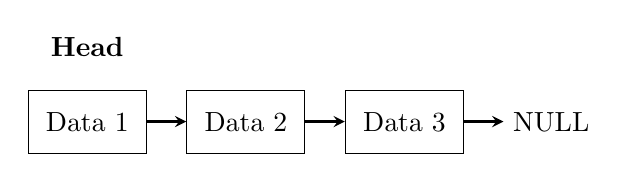
\begin{tikzpicture}[
    node/.style={rectangle, draw, minimum width=1.5cm, minimum height=0.8cm},
    arrow/.style={->, >=stealth, thick}
]
\node[node] (n1) {Data 1};
\node[node, right=0.5cm of n1] (n2) {Data 2};
\node[node, right=0.5cm of n2] (n3) {Data 3};
\node[right=0.5cm of n3] (null) {NULL};

\draw[arrow] (n1) -- (n2);
\draw[arrow] (n2) -- (n3);
\draw[arrow] (n3) -- (null);

\node[above=0.3cm of n1] {\textbf{Head}};
\end{tikzpicture}
\end{center}

\subsection{Complexity Analysis}
\begin{table}[h!]
\centering
\begin{tabular}{|l|c|}
\hline
\textbf{Operation} & \textbf{Time Complexity} \\
\hline
Insert at Head & O(1) \\
Insert at Tail & O(n) \\
Search & O(n) \\
Delete & O(n) \\
Access by Index & O(n) \\
\hline
\end{tabular}
\caption{LinkedList complexity}
\end{table}

\subsection{Usage in Project}
\begin{itemize}[noitemsep]
    \item \texttt{CustomerManager}: Stores registered customers
    \item \texttt{RestaurantManager}: Stores restaurant list
    \item \texttt{DeliveryManager}: Stores delivery agents
    \item \texttt{Restaurant.menu}: Stores menu items
\end{itemize}

\section{Stack}
\subsection{Definition}
A \textbf{Stack} is a LIFO (Last-In-First-Out) data structure where elements are added and removed from the same end (top).

\subsection{Implementation}
\begin{lstlisting}
template <typename T>
class Stack {
    Node<T>* top;
    int count;
public:
    void push(T val);
    void pop();
    T peek();
    bool isEmpty();
    int size();
};
\end{lstlisting}

\subsection{Visual Representation}
\begin{center}
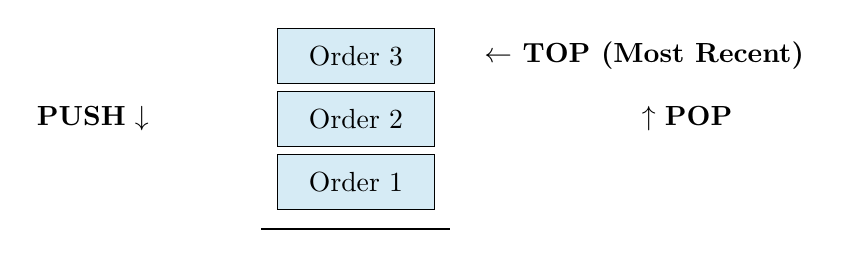
\begin{tikzpicture}[
    box/.style={rectangle, draw, minimum width=2cm, minimum height=0.7cm, fill=secondaryblue!20}
]
\node[box] (e3) at (0,0) {Order 3};
\node[box] (e2) at (0,-0.8) {Order 2};
\node[box] (e1) at (0,-1.6) {Order 1};

\node[right=0.5cm of e3] {\textbf{$\leftarrow$ TOP (Most Recent)}};
\draw[thick] (-1.2,-2.2) -- (1.2,-2.2);

\node[left=1.5cm of e2] {\textbf{PUSH} $\downarrow$};
\node[right=2.5cm of e2] {$\uparrow$ \textbf{POP}};
\end{tikzpicture}
\end{center}

\subsection{Usage in Project}
\begin{itemize}[noitemsep]
    \item \texttt{Customer.orderHistory}: Stores past orders with most recent at top
\end{itemize}

\section{Queue}
\subsection{Definition}
A \textbf{Queue} is a FIFO (First-In-First-Out) data structure where elements are added at the rear and removed from the front.

\subsection{Implementation}
\begin{lstlisting}
template <typename T>
class Queue {
    Node<T>* frontNode;
    Node<T>* rearNode;
    int count;
public:
    void enqueue(T val);
    void dequeue();
    T front();
    bool isEmpty();
    int size();
};
\end{lstlisting}

\subsection{Visual Representation}
\begin{center}
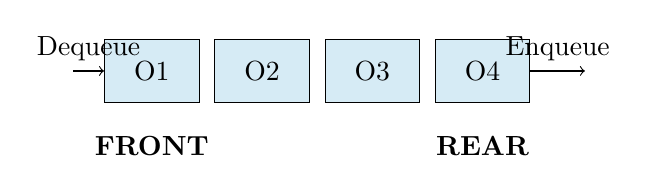
\begin{tikzpicture}[
    box/.style={rectangle, draw, minimum width=1.2cm, minimum height=0.8cm, fill=secondaryblue!20}
]
\node[box] (e1) at (0,0) {O1};
\node[box] (e2) at (1.4,0) {O2};
\node[box] (e3) at (2.8,0) {O3};
\node[box] (e4) at (4.2,0) {O4};

\node[below=0.3cm of e1] {\textbf{FRONT}};
\node[below=0.3cm of e4] {\textbf{REAR}};

\draw[->] (-1,0) -- (e1.west) node[above,midway] {Dequeue};
\draw[->] (e4.east) -- (5.5,0) node[above,midway] {Enqueue};
\end{tikzpicture}
\end{center}

\subsection{Usage in Project}
\begin{itemize}[noitemsep]
    \item \texttt{OrderManager.activeOrders}: Global pending orders
    \item \texttt{Restaurant.pendingOrders}: Restaurant-specific orders
\end{itemize}

\section{Binary Search Tree (BST)}
\subsection{Definition}
A \textbf{BST} is a hierarchical data structure where each node has at most two children, with left child $<$ parent $<$ right child.

\subsection{Implementation}
\begin{lstlisting}
template <typename T>
struct TreeNode {
    T data;
    TreeNode* left;
    TreeNode* right;
};

template <typename T>
class BST {
    TreeNode<T>* root;
public:
    void insert(T val);
    bool search(T val);
    void remove(T val);
    void display(); // Inorder
};
\end{lstlisting}

\subsection{Visual Representation}
\begin{center}
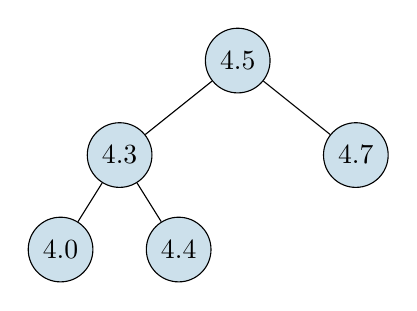
\begin{tikzpicture}[
    level distance=1.2cm,
    level 1/.style={sibling distance=3cm},
    level 2/.style={sibling distance=1.5cm},
    every node/.style={circle, draw, minimum size=0.8cm, fill=primaryblue!20}
]
\node {4.5}
    child {node {4.3}
        child {node {4.0}}
        child {node {4.4}}
    }
    child {node {4.7}};
\end{tikzpicture}

\vspace{0.3cm}
\textit{BST storing restaurant ratings}
\end{center}

\subsection{Usage in Project}
\begin{itemize}[noitemsep]
    \item \texttt{ratingTree}: Stores restaurant ratings for efficient search
\end{itemize}

\section{AVL Tree}
\subsection{Definition}
An \textbf{AVL Tree} is a self-balancing BST that maintains balance by performing rotations when the balance factor exceeds $\pm 1$.

\subsection{Rotations}
\begin{center}
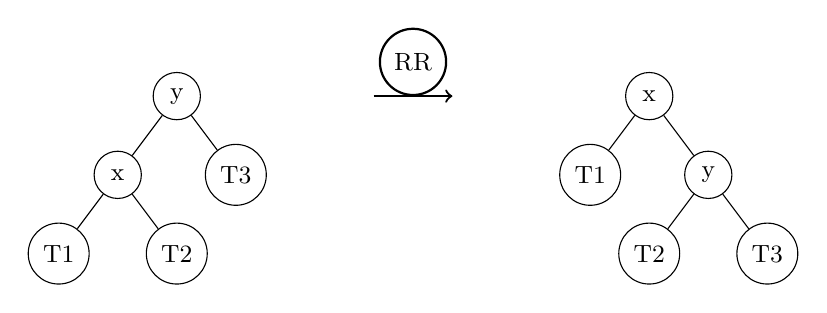
\begin{tikzpicture}[
    every node/.style={circle, draw, minimum size=0.6cm, font=\small},
    level distance=1cm,
    sibling distance=1.5cm
]
% Left tree
\node at (-3,0) {y}
    child {node {x}
        child {node {T1}}
        child {node {T2}}
    }
    child {node {T3}};

\draw[->, thick] (-0.5,0) -- (0.5,0) node[above,midway] {RR};

% Right tree
\node at (3,0) {x}
    child {node {T1}}
    child {node {y}
        child {node {T2}}
        child {node {T3}}
    };
\end{tikzpicture}

\vspace{0.3cm}
\textit{Right Rotation (RR)}
\end{center}

\subsection{Usage in Project}
\begin{itemize}[noitemsep]
    \item \texttt{priceTree}: Stores menu prices with guaranteed O(log n) operations
\end{itemize}

\section{Graph}
\subsection{Definition}
A \textbf{Graph} is a collection of vertices connected by edges. We use an \textbf{adjacency list} representation.

\subsection{Implementation}
\begin{lstlisting}
struct Edge {
    int dest;
    int weight;
};

class Graph {
    int numVertices;
    LinkedList<Edge>* adjLists;
public:
    void addEdge(int src, int dest, int weight);
    LinkedList<Edge>& getAdjList(int vertex);
};
\end{lstlisting}

\subsection{Islamabad Road Network}
\begin{center}
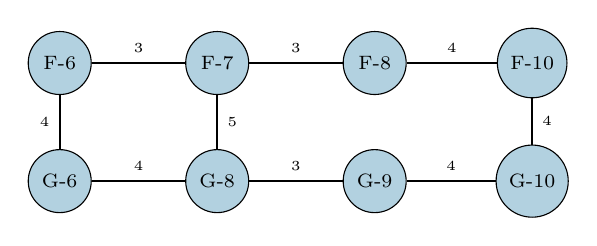
\begin{tikzpicture}[
    node/.style={circle, draw, minimum size=0.8cm, fill=primaryblue!30, font=\scriptsize},
    edge/.style={thick}
]
\node[node] (f6) at (0,0) {F-6};
\node[node] (f7) at (2,0) {F-7};
\node[node] (f8) at (4,0) {F-8};
\node[node] (f10) at (6,0) {F-10};
\node[node] (g6) at (0,-1.5) {G-6};
\node[node] (g8) at (2,-1.5) {G-8};
\node[node] (g9) at (4,-1.5) {G-9};
\node[node] (g10) at (6,-1.5) {G-10};

\draw[edge] (f6) -- (f7) node[above,midway,font=\tiny] {3};
\draw[edge] (f7) -- (f8) node[above,midway,font=\tiny] {3};
\draw[edge] (f8) -- (f10) node[above,midway,font=\tiny] {4};
\draw[edge] (f6) -- (g6) node[left,midway,font=\tiny] {4};
\draw[edge] (f7) -- (g8) node[right,midway,font=\tiny] {5};
\draw[edge] (g6) -- (g8) node[above,midway,font=\tiny] {4};
\draw[edge] (g8) -- (g9) node[above,midway,font=\tiny] {3};
\draw[edge] (g9) -- (g10) node[above,midway,font=\tiny] {4};
\draw[edge] (f10) -- (g10) node[right,midway,font=\tiny] {4};
\end{tikzpicture}

\vspace{0.3cm}
\textit{Partial view of Islamabad sectors graph (distances in km)}
\end{center}

\section{Min-Heap}
\subsection{Definition}
A \textbf{Min-Heap} is a complete binary tree where the parent is always smaller than its children.

\subsection{Implementation}
\begin{lstlisting}
template <typename T>
class Heap {
    T* arr;
    int capacity;
    int currentSize;
    void heapify(int i);
public:
    void insert(T val);
    T extractMin();
    T getMin();
    bool isEmpty();
};
\end{lstlisting}

\subsection{Array Representation}
\begin{center}
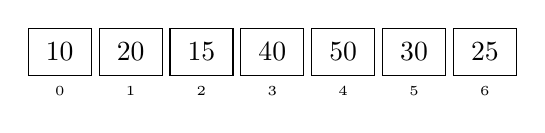
\begin{tikzpicture}[
    box/.style={rectangle, draw, minimum width=0.8cm, minimum height=0.6cm}
]
\foreach \x/\val in {0/10, 1/20, 2/15, 3/40, 4/50, 5/30, 6/25} {
    \node[box] at (\x*0.9, 0) {\val};
    \node[font=\tiny] at (\x*0.9, -0.5) {\x};
}
\end{tikzpicture}

\vspace{0.3cm}
Parent(i) = (i-1)/2, Left(i) = 2i+1, Right(i) = 2i+2
\end{center}

\subsection{Usage in Project}
\begin{itemize}[noitemsep]
    \item Dijkstra's Algorithm: Select minimum distance vertex
    \item Prim's MST: Select minimum weight edge
    \item Kruskal's MST: Sort edges by weight
\end{itemize}

% ============== CHAPTER 3: ALGORITHMS ==============
\chapter{Algorithms}

\section{Dijkstra's Shortest Path Algorithm}
\subsection{Purpose}
Find the shortest path from source to destination sector in Islamabad for optimal delivery routing.

\subsection{Algorithm}
\begin{algorithm}[H]
\caption{Dijkstra's Algorithm}
\begin{algorithmic}[1]
\Function{Dijkstra}{Graph G, source s}
    \For{each vertex v in G}
        \State dist[v] $\gets$ $\infty$
        \State parent[v] $\gets$ NIL
    \EndFor
    \State dist[s] $\gets$ 0
    \State PQ $\gets$ MinHeap()
    \State PQ.insert((s, 0))
    \While{PQ not empty}
        \State (u, d) $\gets$ PQ.extractMin()
        \For{each edge (u, v, w) in G.adj[u]}
            \If{dist[u] + w $<$ dist[v]}
                \State dist[v] $\gets$ dist[u] + w
                \State parent[v] $\gets$ u
                \State PQ.insert((v, dist[v]))
            \EndIf
        \EndFor
    \EndWhile
    \State \Return dist[], parent[]
\EndFunction
\end{algorithmic}
\end{algorithm}

\subsection{Complexity}
\begin{itemize}[noitemsep]
    \item Time: O((V + E) log V) using Min-Heap
    \item Space: O(V)
\end{itemize}

\section{Prim's MST Algorithm}
\subsection{Purpose}
Build optimal delivery network connecting all sectors with minimum total road distance.

\subsection{Algorithm}
\begin{algorithm}[H]
\caption{Prim's Algorithm}
\begin{algorithmic}[1]
\Function{Prims}{Graph G}
    \For{each vertex v in G}
        \State key[v] $\gets$ $\infty$
        \State parent[v] $\gets$ NIL
    \EndFor
    \State key[0] $\gets$ 0
    \State PQ $\gets$ MinHeap()
    \State PQ.insert((0, 0))
    \While{PQ not empty}
        \State u $\gets$ PQ.extractMin().vertex
        \State mstSet[u] $\gets$ true
        \For{each neighbor v of u}
            \If{v not in mstSet and weight(u,v) $<$ key[v]}
                \State key[v] $\gets$ weight(u,v)
                \State parent[v] $\gets$ u
                \State PQ.insert((v, key[v]))
            \EndIf
        \EndFor
    \EndWhile
\EndFunction
\end{algorithmic}
\end{algorithm}

\subsection{MST Visualization}
\begin{center}
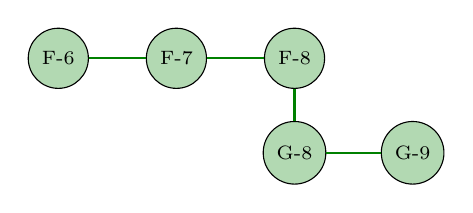
\begin{tikzpicture}[
    node/.style={circle, draw, minimum size=0.7cm, fill=codegreen!30, font=\scriptsize},
    edge/.style={thick, codegreen}
]
\node[node] (f6) at (0,0) {F-6};
\node[node] (f7) at (1.5,0) {F-7};
\node[node] (f8) at (3,0) {F-8};
\node[node] (g8) at (3,-1.2) {G-8};
\node[node] (g9) at (4.5,-1.2) {G-9};

\draw[edge] (f6) -- (f7);
\draw[edge] (f7) -- (f8);
\draw[edge] (f8) -- (g8);
\draw[edge] (g8) -- (g9);
\end{tikzpicture}

\textit{Partial MST connecting sectors}
\end{center}

\section{Kruskal's MST Algorithm}
\subsection{Purpose}
Alternative MST algorithm using Union-Find for cycle detection.

\subsection{Union-Find Operations}
\begin{lstlisting}
int find(int x) {
    if (parent[x] != x)
        parent[x] = find(parent[x]); // Path compression
    return parent[x];
}

void unionSets(int x, int y) {
    int rootX = find(x);
    int rootY = find(y);
    if (rank[rootX] < rank[rootY])
        parent[rootX] = rootY;
    else if (rank[rootX] > rank[rootY])
        parent[rootY] = rootX;
    else {
        parent[rootY] = rootX;
        rank[rootX]++;
    }
}
\end{lstlisting}

\subsection{Complexity}
\begin{itemize}[noitemsep]
    \item Sort Edges: O(E log E)
    \item Union-Find: O($\alpha$(V)) $\approx$ O(1)
    \item Total: O(E log E)
\end{itemize}

\section{Sorting Algorithms}
\subsection{Merge Sort}
\begin{lstlisting}
void mergeSort(T arr[], int left, int right) {
    if (left < right) {
        int mid = (left + right) / 2;
        mergeSort(arr, left, mid);
        mergeSort(arr, mid + 1, right);
        merge(arr, left, mid, right);
    }
}
\end{lstlisting}

\subsection{Quick Sort}
\begin{lstlisting}
void quickSort(T arr[], int low, int high) {
    if (low < high) {
        int pi = partition(arr, low, high);
        quickSort(arr, low, pi - 1);
        quickSort(arr, pi + 1, high);
    }
}
\end{lstlisting}

\subsection{Complexity Comparison}
\begin{table}[h!]
\centering
\begin{tabular}{|l|c|c|c|c|}
\hline
\textbf{Algorithm} & \textbf{Best} & \textbf{Average} & \textbf{Worst} & \textbf{Space} \\
\hline
Merge Sort & O(n log n) & O(n log n) & O(n log n) & O(n) \\
Quick Sort & O(n log n) & O(n log n) & O(n²) & O(log n) \\
\hline
\end{tabular}
\caption{Sorting algorithms comparison}
\end{table}

\section{Searching Algorithms}
\subsection{Linear Search}
\begin{lstlisting}
int linearSearch(T arr[], int n, T key) {
    for (int i = 0; i < n; i++) {
        if (arr[i] == key)
            return i;
    }
    return -1;
}
\end{lstlisting}

\subsection{Binary Search}
\begin{lstlisting}
int binarySearch(T arr[], int n, T key) {
    int left = 0, right = n - 1;
    while (left <= right) {
        int mid = (left + right) / 2;
        if (arr[mid] == key) return mid;
        if (arr[mid] < key) left = mid + 1;
        else right = mid - 1;
    }
    return -1;
}
\end{lstlisting}

\subsection{Comparison}
\begin{table}[h!]
\centering
\begin{tabular}{|l|c|c|}
\hline
\textbf{Algorithm} & \textbf{Time} & \textbf{Requires Sorted} \\
\hline
Linear Search & O(n) & No \\
Binary Search & O(log n) & Yes \\
\hline
\end{tabular}
\caption{Searching algorithms comparison}
\end{table}

% ============== CHAPTER 4: SYSTEM DESIGN ==============
\chapter{System Design}

\section{Architecture Overview}
\begin{center}
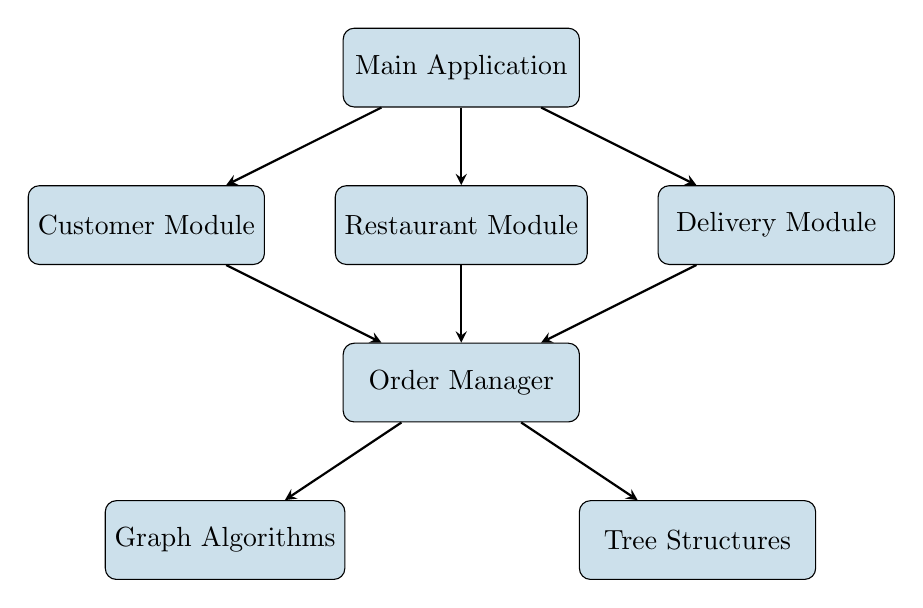
\begin{tikzpicture}[
    module/.style={rectangle, draw, rounded corners, minimum width=3cm, minimum height=1cm, fill=primaryblue!20},
    arrow/.style={->, >=stealth, thick}
]
\node[module] (main) at (0,0) {Main Application};
\node[module] (cust) at (-4,-2) {Customer Module};
\node[module] (rest) at (0,-2) {Restaurant Module};
\node[module] (del) at (4,-2) {Delivery Module};
\node[module] (order) at (0,-4) {Order Manager};
\node[module] (graph) at (-3,-6) {Graph Algorithms};
\node[module] (trees) at (3,-6) {Tree Structures};

\draw[arrow] (main) -- (cust);
\draw[arrow] (main) -- (rest);
\draw[arrow] (main) -- (del);
\draw[arrow] (cust) -- (order);
\draw[arrow] (rest) -- (order);
\draw[arrow] (del) -- (order);
\draw[arrow] (order) -- (graph);
\draw[arrow] (order) -- (trees);
\end{tikzpicture}
\end{center}

\section{Class Diagram}
\subsection{Entity Classes}
\begin{center}
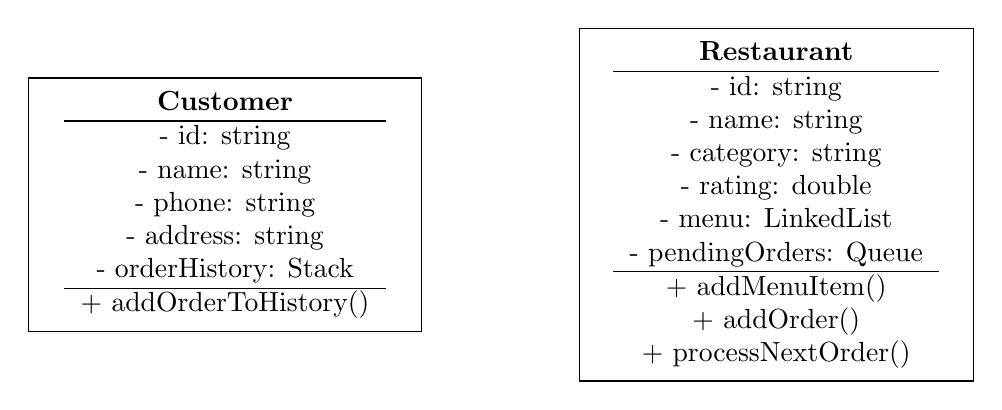
\begin{tikzpicture}[
    class/.style={rectangle, draw, minimum width=5cm, minimum height=3cm}
]
\node[class] (cust) at (0,0) {
    \begin{tabular}{c}
        \textbf{Customer} \\
        \hline
        - id: string \\
        - name: string \\
        - phone: string \\
        - address: string \\
        - orderHistory: Stack \\
        \hline
        + addOrderToHistory()
    \end{tabular}
};

\node[class] (rest) at (7,0) {
    \begin{tabular}{c}
        \textbf{Restaurant} \\
        \hline
        - id: string \\
        - name: string \\
        - category: string \\
        - rating: double \\
        - menu: LinkedList \\
        - pendingOrders: Queue \\
        \hline
        + addMenuItem() \\
        + addOrder() \\
        + processNextOrder()
    \end{tabular}
};
\end{tikzpicture}
\end{center}

\section{Order Flow}
\begin{center}
\begin{tikzpicture}[
    step/.style={rectangle, draw, rounded corners, minimum width=2.5cm, minimum height=0.8cm, fill=secondaryblue!20},
    arrow/.style={->, >=stealth, thick}
]
\node[step] (s1) at (0,0) {Customer Login};
\node[step] (s2) at (3.5,0) {Select Restaurant};
\node[step] (s3) at (7,0) {Add Items};
\node[step] (s4) at (10.5,0) {Place Order};
\node[step] (s5) at (3.5,-1.5) {History (Stack)};
\node[step] (s6) at (7,-1.5) {Queue (Global)};
\node[step] (s7) at (10.5,-1.5) {Queue (Restaurant)};

\draw[arrow] (s1) -- (s2);
\draw[arrow] (s2) -- (s3);
\draw[arrow] (s3) -- (s4);
\draw[arrow] (s4) -- (s5);
\draw[arrow] (s4) -- (s6);
\draw[arrow] (s4) -- (s7);
\end{tikzpicture}
\end{center}

% ============== CHAPTER 5: IMPLEMENTATION ==============
\chapter{Implementation}

\section{File Structure}
\begin{table}[h!]
\centering
\begin{tabular}{|l|l|}
\hline
\textbf{File} & \textbf{Purpose} \\
\hline
main.cpp & Main program and menus \\
LinkedList.h & Generic linked list \\
Stack.h & LIFO stack \\
Queue.h & FIFO queue \\
BST.h & Binary search tree \\
AVL.h & Self-balancing AVL tree \\
Heap.h & Min-heap priority queue \\
Graph.h & Adjacency list graph \\
Dijkstra.h & Shortest path algorithm \\
MST.h & Prim's \& Kruskal's \\
Sorting.h & Merge \& Quick sort \\
Searching.h & Linear \& Binary search \\
Customer.h & Customer entity \\
Restaurant.h & Restaurant entity \\
Order.h & Order entity \\
CustomerManager.h & Customer operations \\
RestaurantManager.h & Restaurant operations \\
OrderManager.h & Order operations \\
DeliveryManager.h & Delivery operations \\
Display.h & Console utilities \\
IslamabadMap.h & ASCII city map \\
\hline
\end{tabular}
\caption{Project files}
\end{table}

\section{Sample Output}

\subsection{Main Menu}
\begin{tcolorbox}[colback=codebg, colframe=gray]
\begin{verbatim}
========================================
   ISLAMABAD FOOD DELIVERY SYSTEM
========================================

 [1] Customer Menu
 [2] Restaurant Menu
 [3] Delivery Menu
 [4] Graph Algorithms (Dijkstra/MST)
 [5] Data Structures Demo
 [0] Exit
----------------------------------------
 Choice: _
\end{verbatim}
\end{tcolorbox}

\subsection{Dijkstra Output}
\begin{tcolorbox}[colback=codebg, colframe=gray]
\begin{verbatim}
=== DIJKSTRA'S SHORTEST PATH ALGORITHM ===

Step 1: Processing F-6 (distance: 0 km)
  -> F-7 (3 km): Distance updated: INF -> 3 km
  -> G-6 (4 km): Distance updated: INF -> 4 km

Step 2: Processing F-7 (distance: 3 km)
  -> F-8 (3 km): Distance updated: INF -> 6 km

=== RESULT ===
Shortest Distance: 14 km
Path: F-6 -> F-7 -> F-8 -> F-10 -> G-10
\end{verbatim}
\end{tcolorbox}

% ============== CHAPTER 6: COMPLEXITY ANALYSIS ==============
\chapter{Complexity Analysis}

\section{Time Complexity Summary}
\begin{table}[h!]
\centering
\begin{tabular}{|l|l|c|}
\hline
\textbf{Operation} & \textbf{Data Structure} & \textbf{Complexity} \\
\hline
Customer Login & LinkedList Search & O(n) \\
Add Restaurant & LinkedList Insert & O(1) \\
Place Order & Queue Enqueue & O(1) \\
View History & Stack Peek & O(1) \\
Search Rating & BST Search & O(log n) avg \\
Search Price & AVL Search & O(log n) \\
Find Route & Dijkstra + Heap & O((V+E) log V) \\
Build MST & Prim's + Heap & O((V+E) log V) \\
Sort Prices & Merge Sort & O(n log n) \\
Search Item & Binary Search & O(log n) \\
\hline
\end{tabular}
\caption{Time complexity summary}
\end{table}

\section{Space Complexity Summary}
\begin{table}[h!]
\centering
\begin{tabular}{|l|c|}
\hline
\textbf{Data Structure} & \textbf{Space} \\
\hline
LinkedList (n items) & O(n) \\
Stack (n items) & O(n) \\
Queue (n items) & O(n) \\
BST (n nodes) & O(n) \\
AVL (n nodes) & O(n) \\
Graph (V vertices, E edges) & O(V + E) \\
Heap (n items) & O(n) \\
\hline
\end{tabular}
\caption{Space complexity summary}
\end{table}

% ============== CHAPTER 7: TESTING ==============
\chapter{Testing}

\section{Test Cases}
\begin{table}[h!]
\centering
\begin{tabular}{|c|l|l|c|}
\hline
\textbf{\#} & \textbf{Test Case} & \textbf{Expected Result} & \textbf{Status} \\
\hline
1 & Customer registration & Added to LinkedList & \checkmark \\
2 & Customer login & Found by phone & \checkmark \\
3 & Place order & Queued correctly & \checkmark \\
4 & View history & Shows most recent & \checkmark \\
5 & Dijkstra F-6 to G-10 & Returns shortest path & \checkmark \\
6 & Prim's MST & Connects all sectors & \checkmark \\
7 & Kruskal's MST & Same weight as Prim's & \checkmark \\
8 & BST search rating & Finds existing rating & \checkmark \\
9 & Merge sort prices & Correctly sorted & \checkmark \\
10 & Binary search item & Returns correct index & \checkmark \\
\hline
\end{tabular}
\caption{Test cases and results}
\end{table}

\section{Compilation}
\begin{tcolorbox}[colback=codebg, colframe=gray]
\begin{verbatim}
$ g++ main.cpp -o main.exe
$ ./main.exe
\end{verbatim}
\end{tcolorbox}

% ============== CHAPTER 8: CONCLUSION ==============
\chapter{Conclusion}

\section{Summary}
This project successfully demonstrates the practical implementation of fundamental data structures and algorithms:

\begin{enumerate}[noitemsep]
    \item \textbf{Linear Structures}: LinkedList, Stack, Queue for data management
    \item \textbf{Trees}: BST and AVL for efficient searching with O(log n)
    \item \textbf{Graphs}: Adjacency list for Islamabad road network
    \item \textbf{Graph Algorithms}: Dijkstra's shortest path, Prim's and Kruskal's MST
    \item \textbf{Sorting}: Merge Sort and Quick Sort with O(n log n)
    \item \textbf{Searching}: Linear and Binary Search implementations
\end{enumerate}

\section{Learning Outcomes}
\begin{itemize}[noitemsep]
    \item Deep understanding of data structure operations and complexities
    \item Practical implementation of graph algorithms for routing
    \item Application of tree structures for efficient data retrieval
    \item Experience with sorting and searching algorithm implementation
    \item Software development skills in C++
\end{itemize}

\section{Future Enhancements}
\begin{itemize}[noitemsep]
    \item Add graphical user interface (GUI)
    \item Implement database persistence
    \item Add real-time order tracking
    \item Integrate GPS coordinates for actual routing
    \item Mobile application development
\end{itemize}

% ============== REFERENCES ==============
\chapter*{References}
\addcontentsline{toc}{chapter}{References}

\begin{enumerate}
    \item Cormen, T. H., Leiserson, C. E., Rivest, R. L., \& Stein, C. (2009). \textit{Introduction to Algorithms} (3rd ed.). MIT Press.
    
    \item Sedgewick, R., \& Wayne, K. (2011). \textit{Algorithms} (4th ed.). Addison-Wesley.
    
    \item Weiss, M. A. (2013). \textit{Data Structures and Algorithm Analysis in C++} (4th ed.). Pearson.
    
    \item Course Lecture Notes - Data Structures \& Algorithms, COMSATS University Islamabad.
\end{enumerate}

\end{document}
